\chapter{LHC-ATLAS実験}
\label{chap_TGC}

% この章では、自分の研究に関連する分野の歴史や現状について説明したり、研究を展開する上で重要となる知識の解説を行います。ここで使用している見出し「ガンマ線天文学…」はあくまで例ですが、もしCherekov Telescope Array(CTA)計画\footnote{省略語は必ず正式名称を先に書き、省略系は丸括弧に入れます。省略語はあくまで「以降このように略す」という用途だからです。また、日本語文章中で使う丸括弧は()ではなく()です。}に携わる院生の書く修士論文であれば、ガンマ線天文学や宇宙線物理学全般について、現行望遠鏡とガンマ線観測の原理について、またCTA計画についての記述がこの章では期待されます。

% 場合によっては「序論」と合体させても良いですが、本章は比較的長くなり結論に直結しない情報もたくさん出てくるため、独立した章である方が読者は読みやすいでしょう。

% またこの章が長くなるときには、例えば「ガンマ線天文学」と「CTA計画」のように、2つの章に分割するというのも良いと思います。\footnote{注意書きの練習です。}


\section{ATLAS検出器}
\label{sec_ATLAS}
    \subsection{ATLAS実験における座標系と変数}


    図\ref{ATLAScordination}にATLAS実験で使われる2種類の座標系を示す。直交座標系は、原点を検出器中心、x軸方向をLHCの中心方向、y軸を地上方向、z軸をビーム軸方向に定義した右手系で定義する。$z>0$ の領域をA side、$z<0$の領域をC sideと呼ぶ。円筒座標系は、ビーム軸を中心とした方位角方向を$\phi$、ビーム軸からの天頂角方向を$\theta$、同型方向を$R$と定義する。$\theta$ 方向を表す変数として擬ラピデティ(Pseudorapidity)$\eta$
    \begin{equation}
        \eta = -\ln(\mathrm{tan}\frac{\theta}{2})
    \end{equation}
    をよく利用する。2粒子の擬ラピデティの差はz軸方向のブーストに対してローレンツ不変であり、物理現象を記述する上で有用だからである。また$\eta$は検出器が覆う領域を説明する際にも利用される。本研究で扱うミューオンシステムでは、|$\eta$| < 1.05の円筒側面領域をバレル領域(barrel)、|$\eta$| > 1.05の円筒底面領域をエンドキャップ(endcap)と呼ぶ。またATLAS実験では粒子の状態を表す物理量としてz軸垂直方向の運動量(横方向運動量,\pt)やエネルギー(横方向エネルギー,$E_{\mathrm{T}}$)を利用する。陽子陽子衝突実験で実行的に衝突するクォークやグルーオンのz軸方向の運動量は不定であるのに対し、ビーム軸に垂直な方向に関しては運動量の和が0であることが保証され、不定性なく再構成できるためである。
    \begin{figure} 
    \centering
    \includegraphics[width=16cm]{fig/Intro/ATLAScordination.pdf}
    \caption[ATLAS検出器における座標系]{ATLAS検出器で用いられる座標系。ビーム軸方向をz軸、LHC中心方向をx軸正の向きとした右手系で定義される。$z>0$をA side、$z<0$をC sideと呼ぶ。円筒座標系も利用され、特に検出器を覆う領域を説明するのに$\eta$が利用される。}
    \label{ATLAScordination}
    \end{figure}
  
    \subsection{ATLAS検出器における超伝導磁石}
    ATLAS検出器では荷電粒子の運動量を測定するため2種類の超伝導磁石が設置されている。図\ref{ATLASmagnet}に各磁石の配置図を示す。ソレノイド磁石は内部飛跡検出器とカロリメーターの間の領域に設置され、内部飛跡検出器内で荷電粒子を曲げる役割をもつ。トロイド磁石はカロリメーターの外側に設置され、内部検出器を透過してきたミューオンを曲げるのに利用される。バレル部とエンドキャップ部のトロイド磁石はお互いの干渉を避けるため22.5度ずらして設置されるが、双方の磁場が影響を与えた結果、eta方向にも$\phi$方向にも均一ではない。そのためミューオンの運動量は飛跡の曲率から直接逆算することが難しく、直線飛跡との角度比較を元に行われる。その方法の詳細は\ref{}説で説明する。

    \begin{figure} 
        \centering
        \includegraphics[width=16cm]{fig/Intro/ATLASmagnet.pdf}
        \caption[超伝導磁石の配置]{超伝導磁石の配置\cite{JINST:2008}。内部飛跡検出器を囲うようにソレノイド磁石が、カロリメーターの外側にトロイド磁石が設置されている。トロイド磁石はバレル部とエンドキャップ部で干渉の内容22.5度ずらして設置される。}
        \label{ATLASmagnet}
    \end{figure}
  
    \subsection{ミューオンスペクトロメーター}
ミューオンスペクトロメーターはATLAS検出器最外層に設置された検出器で、カロリーメーターを透過したミューオンの横方向運動量を測定する役割を担う。ミューオンスペクトロメーターは主にMonitored Drift Tube(MDT)、Resistive Plate Chamber(RPC)、Thin Gap Chamber(TGC)検出器で構成される。RPCとTGCは時間分解能に優れ、応答時間も高速であるためトリガーに利用される。MDTは位置分解能に優れているため、運動量の精密測定に利用される。トロイド磁場内部にはトリガー用の検出器としてTile Calorimeter、TGC EI、RPC BIS78、NSW、が設置されている。

各検出器の設置される領域を図\ref{Muonspectrometer2}に示す。ミューオンスペクトロメーターはトロイドマグネットの磁場構造に合わせて8回対称になっており、マグネットや支持構造と干渉しないよう、$\phi$方向にLarge sector、Small sectorという2種類のsectorに分かれている。トリガー用の検出器として|$eta$| < 1.05のバレル領域ではRPC、1.05 < |$\eta$| < 2.4のエンドキャップ領域ではTGCが最外層に設置される。エンドキャップ領域において磁場内部の検出器カバーする$\eta$、$\phi$領域を図\ref{SL_InnerCoin_covarage}に示す。1.3 < $eta$ < 2.4の領域はNSWが網羅的にカバーしており、1.05 < $eta$ < 1.3領域ではTGC EI、RPC BIS78、Tile カロリメーターがそれぞれ補的にカバーする。

\begin{figure} 
\centering
\includegraphics[width=16cm]{fig/Intro/SL_InnerCoin_covarage.pdf}
\caption[磁場内部の検出器でカバーされる$\eta$、$\phi$領域]{C磁場内部の検出器でカバーされる$\eta$、$\phi$領域\cite{mt_mino}}
\label{SL_InnerCoin_covarage}
\end{figure}

\begin{figure} 
\centering
\includegraphics[width=16cm]{fig/Intro/Muonspectrometer.pdf}
\caption[高輝度LHC-ATLAS実験でのミューオンスペクトロメーターの断面図]{高輝度LHC-ATLAS実験でのミューオンスペクトロメーターの断面図.\cite{tdr_phase2muon_2017017}
}
\label{Muonspectrometer2}
\end{figure}


%TGC検出器
Thin Gap Chamber(TGC)は1.05 < |$\eta$| < 2.4のエンドキャップ領域をカバーする円盤型のミューオントリガー検出器である。TGCはEndcapトロイドマグネットより内側に位置するEndcap Innner(EI)と外側に位置するBig Wheel(BW)に大別される。図\ref{TGC_picture}にBWの写真を示す。TGC BWはz方向に3つのステーションが連なって構成され、衝突点に近い方からM1、M2、M3ステーションと呼ぶ。各ステーションは2層または3層のガス層で構成されており、2層のものをdoublet、3層のものをtripletと呼ぶ。BWではM1がtriplet、M2、M3がdoubletである。

\begin{figure} 
\centering
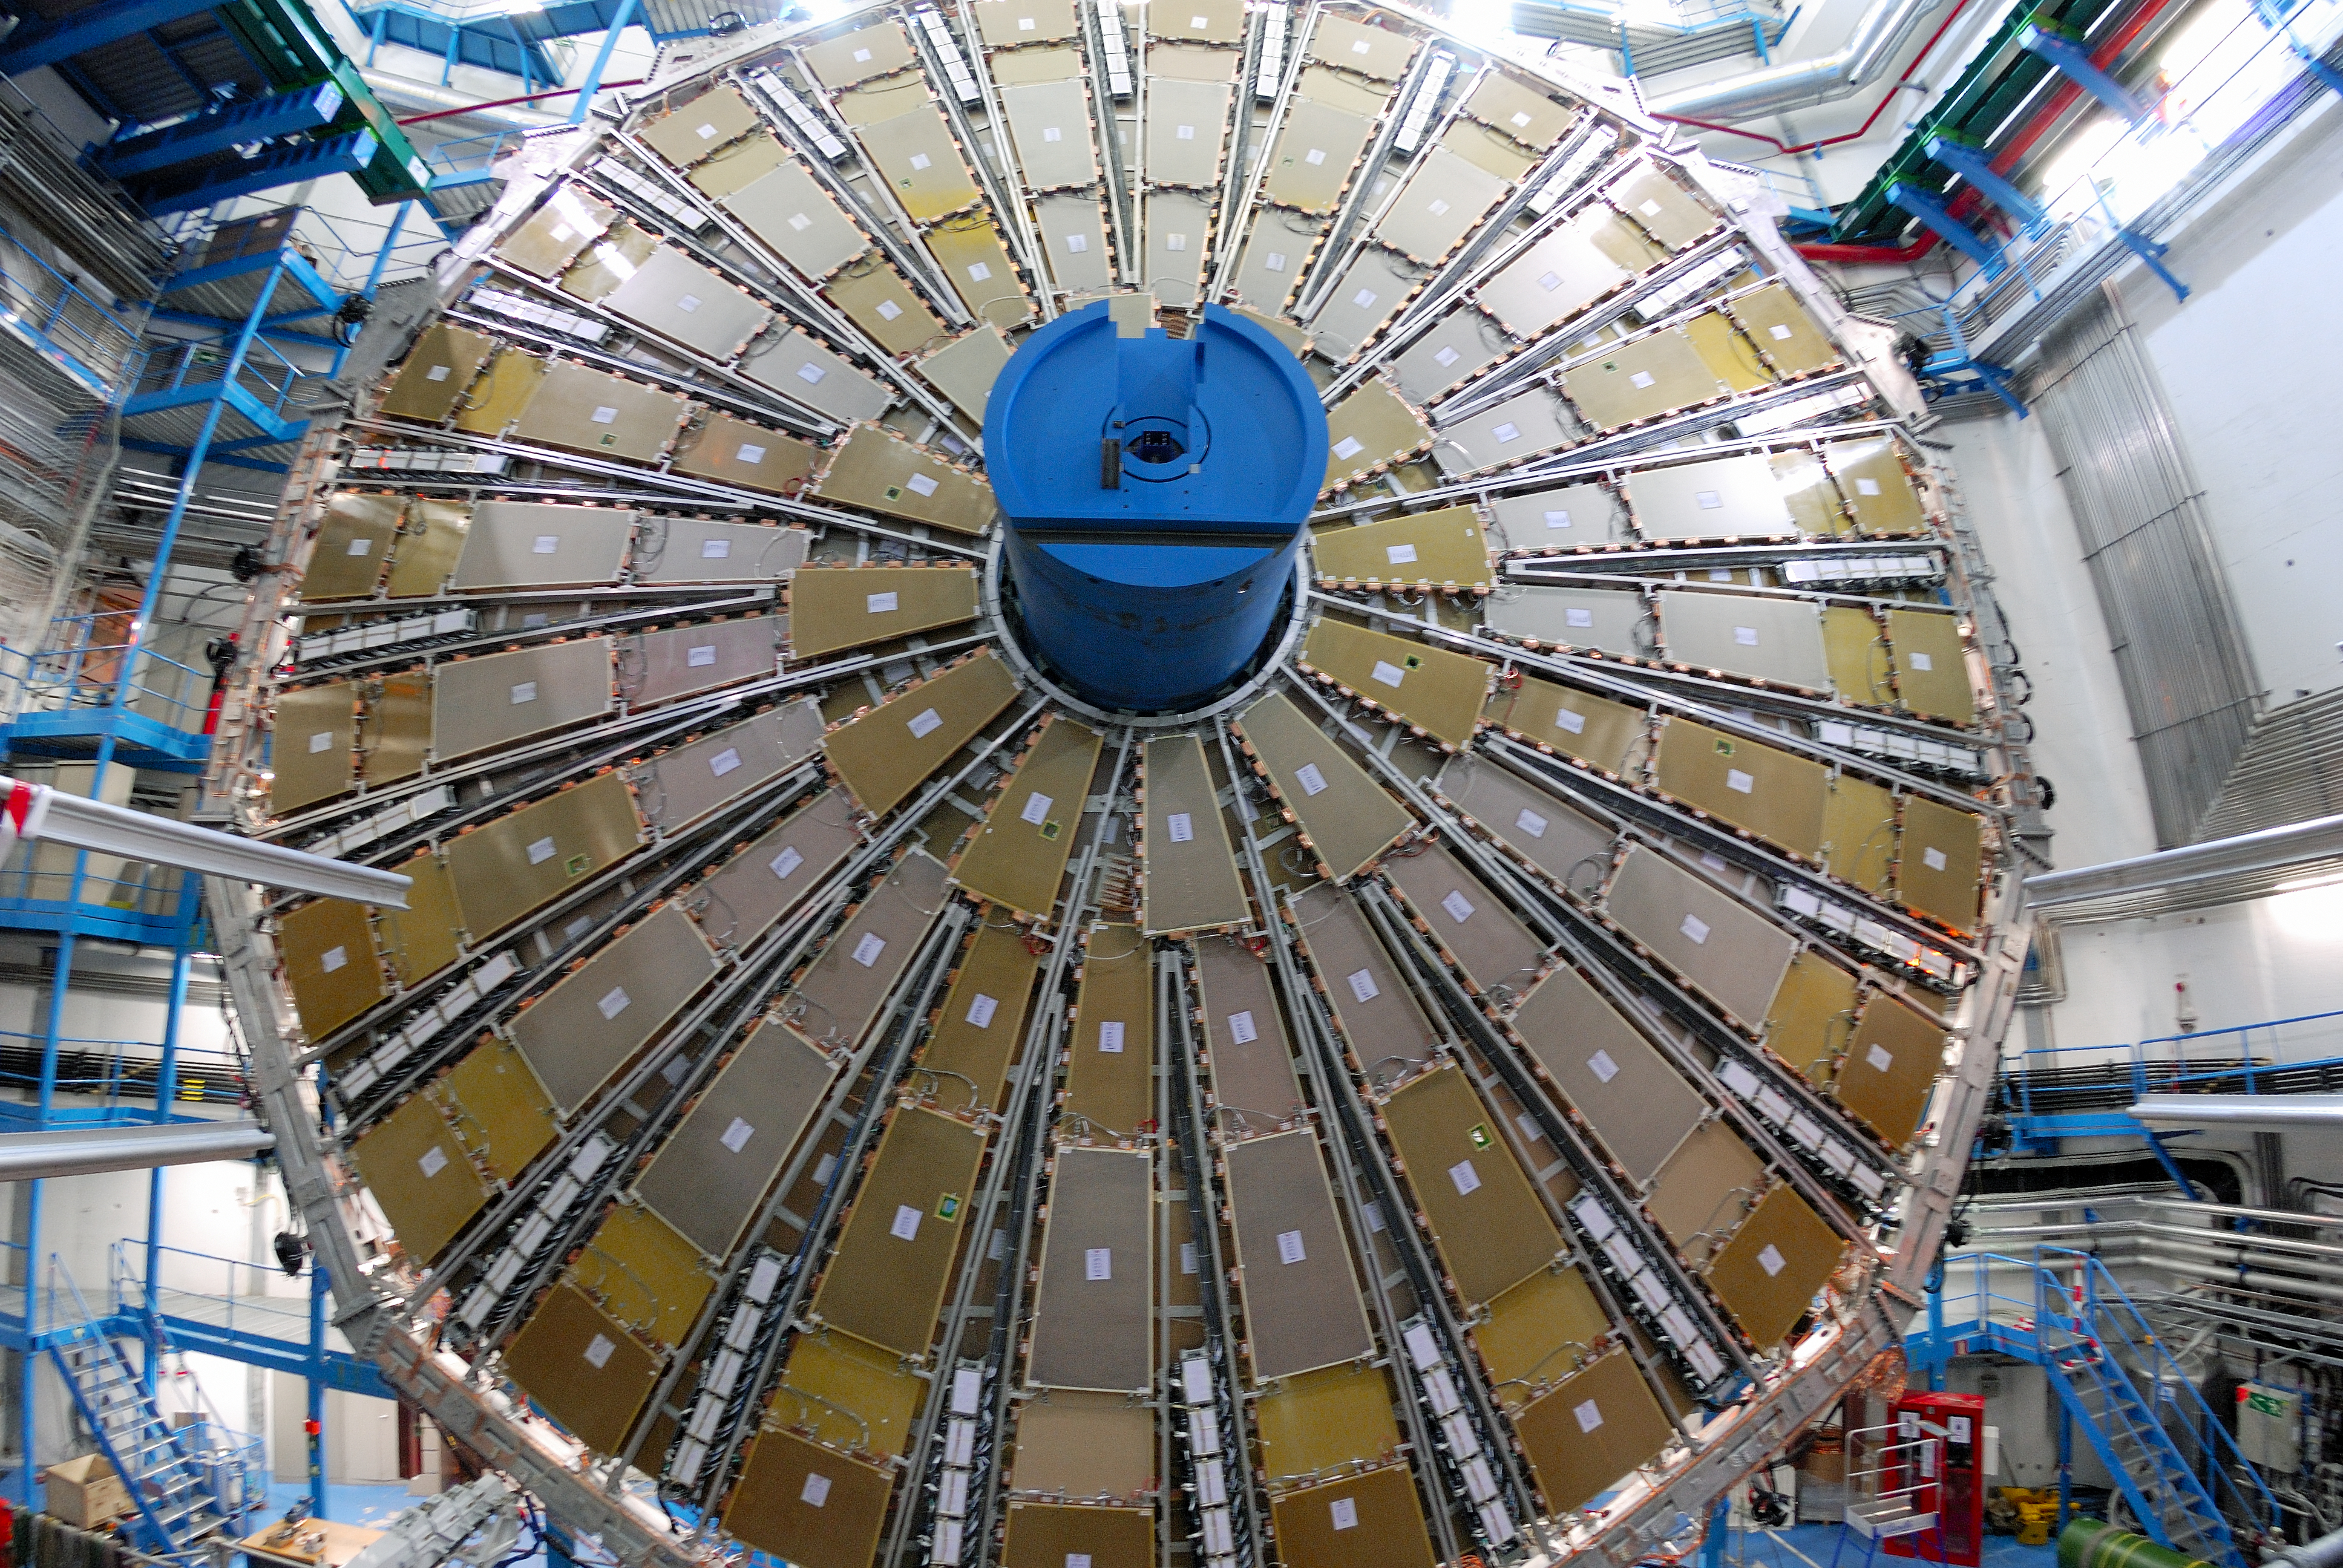
\includegraphics[width=16cm]{fig/Intro/TGC_picture.jpg}
\caption[TGC検出器]{TGC検出器の正面写真(M1)\cite{cern_document_server}}
\label{TGC_picture}
\end{figure}

TGCチェンバーの構造を図\ref{TGC_structure}に示す。TGCはアノードワイヤー間隔が1.8mm、アノードとカソードストリップの間隔が1.4 mmであるMWPCである。ワイヤーはR方向、ストリップは$\phi$方向に直交して張られており、2次元位置を読み出しが可能である。ガス層には$CO_2/n-C_5H_{12}$が55:45で混合されたガスが充填されている。

\begin{figure}
\begin{minipage}[b]{.5\linewidth}
\centering
\includegraphics[height=5cm]{fig/Intro/TGC_structure.pdf}
\subcaption{TGCチェンバーの断面図}
\end{minipage}%
\begin{minipage}[b]{.5\linewidth}
\centering
\includegraphics[height=5cm]{fig/Intro/TGC_crosssection.pdf}
\subcaption{TGC doubletとtripletの断面図}
\end{minipage}%
\caption[TGCチェンバーの断面図]{(a)はTGCチェンバーの断面図を表す\cite{JINST:2008}。ワイヤーとストリップが直交して張られていることがわかる。(b)はTGC doubletとtripletの断面図である。それぞれ2層、3層のガスギャップで構成されており、各ガスギャップの間はペーパーハニカムにより満たされている。}
\label{TGC_structure}
\end{figure}


荷電粒子がTGCに入射すると、荷電粒子によりガス分子が電離される。電離した電子はワイヤーに印加された2.8 kVの電圧によりワイヤー方向に集められ、ワイヤー付近に到達すると強い電場により電子雪崩を生じる。ワイヤーでは電子雪崩で生じた正イオンのドリフトが、ストリップではそれらの鏡像電荷が電流信号として検出される。

TGC検出器はトリガー用の検出器であり、ガスギャップが薄く、ワイヤー間隔が小さいため時間応答がよい。これにより陽子衝突頻度である25nsより細かな時間分解能でミューオンを検出し、そのミューオンがどの陽子バンチ衝突に由来するのかを識別(Bunch Crossing IDentification, BCID)することができる。一方、TGC検出器はそれほど高い位置分解能が求められていないため、ワイヤー電極を4 ~ 20本まとめてから読み出しを行う。結果としてワイヤー、ストリップは合計32万チャンネルをもつ。

\begin{itembox}{要修正}
    一時的に青木さんの丸パクリしてる。
\end{itembox}

BWの外側(1.05 < |$\eta$| < 1.92)はエンドキャップ領域、円盤の内側(1.92 < |$\eta$|< 2.4)はフォワード領域と呼ばれる。エンドキャップ領域では$\phi$方向に48回対称になるよう、フォワードでは$\phi$方向に24回対称になるようにチェンバーが設置されている。エンドキャップ領域の1/48、フォワードの1/24はトリガー回路的に独立しており、そrぞれが"トリガーセクター"と呼ばれる。
また電源供給、ガス供給、電気回路制御、読み出しの観点からBWは$\phi$方向に12個のセクターに分割される。各"1/12セクター"はx軸の正の方からy軸の正の方向に向かって順にA-sideではA01からA12、C-sideではC01からC12までの名前がついている。



\section{ATLAS実験におけるTDAQシステム}
\label{sec_TDAQ}
   
    \subsection{Run3でのTDAQシステム}
    \label{subsec_run3TDAQ}
    \ref{chap_Intro}節で述べたようにLHCでは25 nsの間隔で陽子バンチが衝突するため、衝突で生じたすべてのデータを保存することはできない。限られた読み出し帯域とオフラインの計算リソースを最大限有効活用するためには興味のある衝突事象のみを記録するトリガーが重要となる。またトリガー判定がなされたイベントに対して正しくデータを取得するには、トリガーシステムとデータ取得(data acquisition,DAQ)システムが連動して機能する必要がある。ATLAS実験では、トリガーとデータ取得をまとめてTrigger and Data Acquisition(TDAQ)システムと呼ぶ。図\ref{Run3_TDAQ}にRun3におけるTDAQシステムの概要を示す。ATLASのトリガーシステムはLevel-1という初段のハードウェアトリガーと、それに続くHigh Level Trigger(HLT)という後段のソフトウェアトリガーから構成される。

    \begin{figure} 
    \centering
    \includegraphics[width=16cm]{fig/Intro/Run3_TDAQ.pdf}
    \caption[Run3におけるTDAQシステムの概要]{Run3におけるTDAQシステムの概要\cite{Run3_TDAQ}。トリガーシステムはLevel-1 Triggerという初段ハードウェアトリガーとHigh Level Trigger(HLT)という後段のソフトウェアトリガーから構成される。L1 TriggerはL1 CaloとL1 Muonに大別されCTPで総合的なトリガー判定がなされる。L1 TriggerをパスしたイベントはHLTでより精度の高いトリガー判定が行われ、CERN Permanent Strageに保存される。 }
    \label{Run3_TDAQ}
    \end{figure}

    \subsubsection{Level-1 Trigger}
    \vskip0.5\baselineskip
    Level-1 Triggerは25 ns間隔で行われるすべての陽子バンチ衝突事象の中から、物理的に興味のあるオブジェクトを含むイベントを大まかに選別する初段トリガーである。L1 Triggerによってイベントレートは40 MHzから100 kHzまで削減される。L1 Triggerは大量のデータを高速で処理する必要があるため、ASICやFPGAなどのハードウェアを利用したトリガー判定が行われる。
    ATLASでのL1 Triggerシステムは主にLevel-1 CaloとLevel-1 Muonで構成される。Level-1 Caloはカロリーメーターからのエネルギー情報をもとに発行されるトリガーで、高いエネルギーを持つ電子、光子、ジェットを含むイベントに対してトリガーが発行される。Level-1 Muonは主にRPCとTGCからの情報をもとに発行されるトリガーで、横方向運動量の大きなMuonを含むイベントに対してトリガーが発行される。これらの信号はCentral Trigger Processor(CTP)に渡され、総合的にLevel-1トリガー判定が行われる。L1 Triggerが発行されると各検出器のフロントエンド回路にはLevel-1 Accept(L1A)が送られ、そのバンチ衝突に由来する検出器のヒット信号がReadout Driver(ROD)へと送られる。
    Level-1 Triggerではバンチ衝突が生じてからL1Aが届けられるまでの時間(Level-1 レイテンシー)が一定であるFIxed Latency Schemeを採用している。陽子バンチ衝突で生じるデータはL1Aが出されるまでの間、各フロントエンドエレクトロニクス上のバッファーに保管される。L1レイテンシーは設置可能なバッファーサイズによって制限されており、Run3では2.5 $\mu\mathrm{s}$に設定されている。

    \subsubsection*{High Level Trigger(HLT)}
    \vskip0.5\baselineskip
    HLTは初段トリガーをパスしたイベントから最終的にストレージに保存する事象を選ぶ役割を担う、ソフトウェアベースのトリガーである。初段トリガーでは使われなかった内部飛跡検出器やMDTなどのミューオン精密測定用検出器からの情報も利用して、より高い精度でイベント再構成を行う。HLTによりトリガーレートは1kHzまで削減され、記録すべきと判断されたイベントは、永久保存のためにCERNのコンピューティングセンターであるTier-0へ送られる。

    \subsubsection*{トリガーメニュー}
    ATLAS実験は陽子陽子衝突で生じるさまざまな事象を取得することで、幅広い終状態を持つ多様な物理解析を展開する。そのためにも、広範な物理事象を取得できるよう限られたトリガーレートを適切に分配する必要がある。そのために用意されているのが図\ref{Run2_Triggermenu}に示すようなトリガーメニューである。トリガーメニューでは、解析で利用されるlepton、jet、消失横方向エネルギー($E_{\mathrm{T}^{\mathrm{miss}}}$)などの典型的なオブジェクトを取得するためのLevel-1およびHLTトリガーの閾値が定められる。またそれに伴いトリガーレートのシミュレーションも行われ、全体を通してトリガーレートの制約を守るよう設計される。

    \begin{figure} 
    \centering
    \includegraphics[width=16cm]{fig/Intro/Run2_Triggermenu.pdf}
    \caption[Run2でのトリガーメニューの一例]{Run2でのトリガーメニューの一例\cite{Run2_Triggermenu}。解析で利用される典型的なオブジェクトを取得するためのLevel-1およびHLTでのトリガー閾値が定められる。全体を通してトリガーレートの制約を守るよう設計される。}
    \label{Run2_Triggermenu}
    \end{figure}

    \subsection{高輝度LHC-ATLAS実験でのTDAQシステム}
2029年からビーム輝度を約3倍に増強した高輝度LHC実験が始まる。高輝度LHC実験ではパイルアップによる背景事象が大幅に増加し、結果としてトリガーレートが増加する。\ref{}で述べたように、現行のTDAQシステムを維持しつつ読み出しレートの制約を守るためには、興味のある物理事象へのアクセプタンスを落とすことにつながる。そこで高輝度LHC実験に向けて大規模なTDAQシステムのアップグレードが行われる。高輝度LHC実験では初段トリガーのレートは100 kHzから1 MHzへ、後段のトリガーレートは1 kHzから10 kHzへと拡張される。さらに、初段トリガーレイテンシーも2.5 $\mu\mathrm{s}$から10 $\mu\mathrm{s}$へと拡張される。これにより洗練されたトリガーアルゴリズムを実装することができるようになる。図\ref{Phase2_TDAQ}に高輝度LHC実験でのTDAQシステムの概要を示す。
高輝度LHC実験では初段トリガーをLevel-0 Trigger、後段トリガーをEvent Filter(EF)と呼ぶ。

\begin{figure}
\begin{minipage}[b]{.5\linewidth}
\centering
\includegraphics[height=7cm]{fig/Intro/Phase2_L0trigger.pdf}
\subcaption{Level-0 Triggerシステムの概要}
\end{minipage}%
\begin{minipage}[b]{.5\linewidth}
\centering
\includegraphics[height=7cm]{fig/Intro/Phase2_EF.pdf}
\subcaption{Event FilterとDAQシステムの概要}
\end{minipage}%
\caption[高輝度LHC-ATLAS実験におけるTDAQシステムの概要]{高輝度LHC-ATLAS実験におけるTDAQシステムの概要\cite{tdr_phase2tdaq_2017020}。(a)にLevel-0 Triggerシステムの概要を示す。Level-0 TriggerはLevel-0 CaloとLevel-0 Muonに大別され、それぞれCTPで総合的なトリガー判定がなされる。CTPで後段に送られるべきと判断された場合、FELIXを経由して各フロントエンドエレクトロニクスにL0A信号が分配される。(b)にEvent FilterとDAQシステムの概要を示す。L0Aを受けた各システムは検出器からのヒットデータをFELIXに送る。FELIXは受け取ったデータをEvent Filterに渡す。EFではソフトウェアベースのトリガー判定が行われ、最後まで残ったデータがCERNのPermanent Strageに保存される。}
\label{fig_formats}
\end{figure}

L0 TriggerはL0 Calo、L0 Muon、Global Trigger、CTPで構成される。L0 Muonでは、新たに精密測定用のMDTもトリガーに用いられる。TGCやRPCの情報と組み合わせることでより精度の高いトリガー判定を実現する。Global TriggerはL1 CaloとMUCTPIからの位置や\pt、\Et などの情報を基に、特徴的なトポロジーを持つ事象を選び出してCTPに送る。CTPはトリガーメニュー(図\ref{Phase2_Triggermenu})に従い、各トリガー条件に指定されたプリスケーリングファクターを適用してトリガー判定を行う。各フロントエンドエレクトロニクスにはFront-End Link eXchange (FELIX) を経由してLevel-0 Accept(L0A)信号が分配される。L0Aを受けた各エレクトロニクスは該当する検出器ヒット情報をFELIXに送り返す。FELIXはこれらのデータをEvent Filterに転送する。Event Filterではソフトウェアのトリガー判定が行われトリガーレートは10 kHzまで削減される。最終的に残ったデータは、CERNの永久ストレージに保存される。

\begin{figure} 
\centering
\includegraphics[width=16cm]{fig/Intro/Phase2_Triggermenu.pdf}
\caption[高輝度LHCにおけるトリガーメニューの例]{高輝度LHCにおけるトリガーメニューの例\cite{tdr_phase2tdaq_2017020}。解析に利用される典型的なオブジェクトに対してL0 TriggerおよびEvent Filterでのトリガーレートが分配されている。L0 TriggerレートはRun3の約10倍、Event Filterでのレートは約6倍に増強される。}
\label{Phase2_Triggermenu}
\end{figure}



\section{TGC検出器トリガーシステム}
\label{sec_TGCtrigger}

    \subsection{TGCトリガーのコンセプト}

衝突点からエンドキャップ方向(1.05 < |$\eta$| < 2.4)に飛来するミューオンはエンドキャップトロイド磁石で曲げられ、TGC検出器に入射する。TGC検出器各層ではワイヤー、ストリップの2次元読み出しにより(R、$\phi$)2次元座標が検出される。TGC検出器はz方向に3つのステーションを有しており、3ステーション間のコインシデンスをとることでミューオンの3次元飛跡を再構成し、運動量を概算する。TGC検出器における運動量概算手法のコンセプトを図\ref{TGC_triggerconcept}に示す。

\begin{figure} 
\centering
\includegraphics[width=16cm]{fig/Intro/TGC_triggerconcept.pdf}
\caption[TGCにおけるトリガーのコンセプト]{TGCにおけるトリガーのコンセプト\cite{mt_akatsuka}。ミューオンが実際に残したヒット点と無限運動量飛跡の位置の差分($\mathrm{dR}$,$\mathrm{\phi}$)を利用して\pt を概算する。}
\label{TGC_triggerconcept}
\end{figure}

内部飛跡検出器では、磁場で曲げられた粒子の曲率半径を利用して運動量を測定する。一方、TGC検出器自体には磁場がかけられておらず、ミューオンはTGC検出器を直線的に通過するためこの手法は利用できない。そこでTGC検出器では3ステーションのヒットから再構成したミューオンの飛跡と、M3のヒット点と衝突点を直線的結んだ無限運動量飛跡のを比較することで\pt を概算する。具体的には、ミューオンが実際に残したヒット点と無限運動量飛跡のM1及びM2の交点との位置の差分($\mathrm{dR}$,$\mathrm{\phi}$)を利用する。\pt が小さいミューオンほどトロイド磁場領域で大きく曲げられるため、$\mathrm{dR}$ 及び $\mathrm{\phi}$は大きくなる。
\ref{}節で述べたようにエンドキャップトロイド磁石から作られる磁場とバレルトロイド磁石で作られる磁場は互いに干渉しており、エンドキャップ領域に張られる磁場は、$\phi$方向の成分だけでなくR方向にも成分をもつ。そのため衝突点から飛来するミューオンはR方向だけでなく$\phi$方向にも曲げられる。また磁場が一様でないため、($\mathrm{dR}$,$\mathrm{\phi}$)とpTの関係はミューオンの飛来する場所に依存する複雑な関数となり、代数的に求めるのが困難である。そこであらかじめシミュレーションを用いて、($\mathrm{dR}$,$\mathrm{\phi}$)とPtの関係性をまとめたテーブル(Look Up Table、LUT)を領域ごとに用意する。これにより再構成した($\mathrm{dR}$,$\mathrm{\phi}$)をもとにLUTに問い合わせることで高速でpTを計算することができる。

加えて、Run2以降のトリガーロジックではTGC BWの情報で得られたミューオン候補はエンドキャップトロイド磁場内部に位置する検出器とコインシデンスがとられる。このコインシデンスをInner Coincidenceと呼ぶ。これにより図\ref{}に示すようなフェイクトリガーと呼ばれる、衝突点に由来しない荷電粒子によるトリガーを削減することが期待される。フェイクトリガーの発生源としては陽子陽子衝突やハドロンカロリメーター内で生じた中性ハドロンが、トロイド磁石と衝突して荷電粒子を吐き出す事象などが考えられる。またNSWなど位置分解能に優れた検出器からの情報を組み合わせてptを計算することでTGC BW単体で計算するよりptの計算精度を高めることができる。

このpTに対して閾値を設け、それ以上のpTを持つミューオンを含む事象を選別する。

    \subsection{Run3でのTGCトリガーシステム}
上記のトリガーのコンセプトを実現するRun3 TGCシステムにおけるTDAQシステムのブロック図を図\ref{TGC_run3tdaq}に示す。

\begin{figure} 
\centering
\includegraphics[width=16cm]{fig/Intro/TGC_run3tdaq.pdf}
\caption[Run3におけるTGC TDAQシステム]{Run3におけるTGC TDAQシステム}
\label{TGC_run3tdaq}
\end{figure}

図の赤色の線はトリガーパス、青色はデータパスを示す。

TGC検出器にミューオンが入射すると、\ref{}節で述べたように各ガスレイヤーに張られたワイヤー、ストリップにアナログの電流信号が発生する。アナログ信号はTGC検出器に直接取り付けられたAmplifier Shaper-Discriminator(ASD)に集められる。ASDでは信号を増幅、整形し、閾値電圧と比較することでデジタル信号に変換される。デジタル信号は後段のPS board上に搭載されたPatch-Panel ASIC(PPASIC)において、ミューオンの飛行時間の違いやASDからPS boardに至るケーブルの長さの違いに起因する、チャンネルごとの信号到達時間の差を調整し、各デジタル信号がどのバンチ陽子衝突に由来するのか識別する(BCID)。この後から信号はトリガーパスとリードアウトパスに分けられる。

トリガーパスはSlave Board(SLB)、High-pt(HPT)ボード、Sector Logic(SL)というパスを辿る。SLBではワイヤーとストリップそれぞれでM1ステーション内およびM2、M3間のコインシデンスがとられ、($\mathrm{dR_{23}}$,$\mathrm{\phi_{23}}$)が計算される。M1では3層中2層以上のコインシデンスが、M2、M3では4層中3層以上のヒットが要求され、コインシデンスが取れたもののうち検出位置の差が小さいものを絞って出力する。High-pT(HPT)ボードではM1、M3間のコインシデンスがとられ($\mathrm{dR_{13}}$,$\mathrm{\phi_{13}}$)が計算され、絶対値の小さいもの(高いpTを持った)から出力される。SLボードではM3におけるヒット位置および($\mathrm{dR_{13}}$,$\mathrm{\phi_{13}}$)をもとにワイヤー・ストリップ間のコインシデンスがとられ、LUTをもとにptを概算する。また磁場内部に位置する検出器(NSW、RPC BIS78、TGC EI、Tile カロリメーター)の飛跡情報ともコインシデンスがとられ、より精度の高いptが計算される。SLで得られた入射位置とpt情報はMUon-to Central Trigger Processor Interface(MUCTPI)に送られCTPへpT情報が渡される。CTPで後段へ送るべきと判断された場合にはL1A信号が発行される。

読み出しパスはSLB、Star SWitch(SSW)ボード、ReadOut Driver(ROD)というパスを辿る。PPASICで同期された信号はトリガー判定が完了するまで、SLB内のL1Bufferに一時的に保存される。SLBでは最大128イベント分の信号をバッファーすることができる。\ref{}節で述べたようにL1-TriggerはFixed latency schemeを採用しており、L1 Bufferにデータが入ってからそのイベントにL1Aが出されるまでの時間は固定である(L1-latency)。そのためSLBはL1Aを受けた後、L1 latencyだけ前のデータを読み出すことで正しくL1Aに対応するデータを読み出すことができる。SLBから読み出されたデータはSSWボードでゼロサプレスと呼ばれるデータ圧縮を行い、イベント毎にパッケージする(Event Building)。RODは1つのセクター内の全てのSLB-SSWから送られるすべてのデータをまとめ、さらに後段のReadOut System(ROS)へとデータを送信する。

これらのTGCエレクトロニクスのうち、ASD、PS board、HPT、SSWはフロントエンドエレクトロニクスと呼ばれ、UX15というTLAS実験室内に設置される。

ASDはTGCチェンバーに直接取りつけたアダプタボードにマウントされる。PS boardは2枚毎にアルミケース(PS-pack)に収納され、TGCチェンバー付近に設置される。HPTおよびSSWは、BWの外側のMini-Rack内のVMEクレートに収められる。

SL、ROD以降バックエンドエレクトロニクスと呼ばれUX15から100 mほど離れたUSA15というATLAS回路室内に設置される。HPTからSLおよびSSWからRODへの通信はUX15とUS15間の限られた帯域幅を用いて行う必要があり、高輝度LHC-ATLAS実験ではG-linkと呼ばれる旧式のシリアル通信規格で接続している。G-linkにおけるシリアルデータの転送レートは約1 Gpbsである。

次にTTC系について述べる。

Level 1 Buffer以前の読み出し回路およびトリガー回路はFixed latency schemeを実現するためにLHCの陽子バンチ衝突と同期して動作する必要がある。このために各検出器とLHCを同期するためのシステムをTiming, Trigger and Control (TTC)システムとよび、そのために配布される信号をTTC信号と呼ぶ。TTC信号には陽子バンチ衝突と同期した40.079 MHzのクロックであるLHCバンチ交差クロックやL1A信号などが含まれる。Run3でのTTC系の概要を図\ref{}に示す。TTC信号はCTPから各検出機サブシステムのLocal Trigger Processor(LTP)に配られる。その後TTC信号はTTCvi, TTCex、TTXrx と呼ばれる TTC 専用モジュール及び TTC 専用線を用いて PS board, HPT, SSW, SL へ分配される。

\begin{figure} 
\centering
\includegraphics[width=16cm]{fig/Intro/Run3_TTC.png}
\caption[Run3 TGCシステムにおけるTTCシステムの概要]{Run3 TGCシステムにおけるTTCシステムの概要\cite{JINST:2008}}
\label{Run3_TTC}
\end{figure}

\begin{itembox}{要修正}
    モロパクリ
\end{itembox}
以上で述べたRun3のTDAQシステムでは高輝度LHC-ATLAS実験におけるトリガー・読み出し性能の要求を満たすことができない。限界は主にSLBに設置されるL1 Bufferの大きさとATLAS実験室と回路しつの間の帯域幅からきている。Run3のL1 Bufferは最大128イベント分のデータしか保存することができないため、高輝度LHC-ATLAS実験のL0-latencyの要求10us(400バンチ)の間データを保持しておくことができない。また1 MHzの初段トリガーレートを満たす量のデータを読み出すには、現行システムでのATLAS実験室とATLAS回路質間の帯域幅では不十分である。
フロントエンドエレクトロニクスの設置場所を図\ref に示す。

    \subsection{高輝度LHC-ATLAS実験でのTGCトリガーシステム}  
前節で述べた困難を克服するため、高輝度LHC-ATLAS実験に向けてTGC検出器エレクトロニクスシステムは大幅にアップグレードされる。主な違いはPS boardでBCIDされたすべてのヒット信号がトリガーをかけられることなく後段のSLに送られることである。Run3のトリガーパスではSLBボードやHPTボードでコインシデンスをとることで、TGCからのヒット信号はデータサイズを徐々に減らしながら回路室へ送られる。高輝度LHC-ATLAS実験では新しく高速シリアル通信技術を導入することで、実験室と回路室の間の帯域幅を1 Gbps程度から10 Gbpsへ大幅に拡張する。これにより、PS boardで受け取ったTGCからの信号を、削減することなくすべて回路室のSLへ転送することが可能になった。回路室ではボードのサイズや放射線への堅牢性に対する制約がないため、バックエンドエレクトロニクスであるSLには大規模なFPGAを搭載することができる。その結果、CTPからL0Aが発行されるまでデータを保管しておくL0バッファーも余裕を持って実装することができ、10 usのL0レイテンシーに対応することができる。またSLは1つのトリガーセクター内の全てのPS boardからのヒット信号を集約するため、TGC BW 7層分の情報を利用したより包括的なトリガーアルゴリズムを実現することができる。高輝度LHC-ATLAS実験でのトリガーロジックの詳細は\ref{}節で示す。

図\ref{TGC_phase2tdaq}に高輝度LHC-ATLAS実験でのTGC検出器エレクトロニクスの概要を示す。ASDは現行システムのものをそのまま用いる。一方Run3で使われていたPS board、SLB、HPT、SLは全て撤廃され、新しくPrimary ProceSsor board(PS board)、JTAG AssisTance Hub(JATHub)、TAM(Timing Alignment Master)、Endcap Sector Logic(SL)が設置される。PS boardはRun3と同様のPS-packに格納され、TGC検出器付近に設置される。JATHubとTAMはMini-pack内のVMEクレート内に設置される。SLはUSA15に設置される。1つのSLはTGCの1/24セクター担当し、このセクターを担当する最大31枚のPS boardからヒットデータを受け取る。

\begin{figure} 
\centering
\includegraphics[width=16cm]{fig/Intro/TGC_phase2tdaq.pdf}
\caption[高輝度LHC-ATLAS実験におけるTGC検出器システムの概要]{高輝度LHC-ATLAS実験におけるTGC検出器システムの概要\cite{tdr_phase2muon_2017017}}
\label{TGC_phase2tdaq}
\end{figure}

トリガーパスにおけるデータの伝達を赤色の矢印で示す。TGCで生じた電流信号はASDで電圧信号に変換されたのち、PS board上のPP ASICでタイミングが揃えられ、BCIDされる。PP ASICからの信号はヒットの有無に関わらずPS board上のFPGAから光ファイバーを通じてSLに送信される。SLはTGC BW、TGC EI、NSW、RPC BIS78、Tile カロリメーターの情報を用いてミューオンのptを概算する。その後SLはMDT Trigger Processorにミューオン飛跡候補を送信し、よりよいpt分解能の情報を得る。SLからのトリガー出力はMUCTPI通じてCTPへ送信される。

CTPでのトリガー判定を待っている間のデータのバッファーもSLで行われる。SLはL0Aを受けると、そのイベントに該当するデータをFELIXを通じて後段に送信する。

TTC信号はCTPからFELIXを通してSLに分配される。SLはPS boardへのコントロール信号に乗せてTTC信号を分配する。

このシステムではバックエンドのSLとフロントエンドのPS boardは光リンクだけで接続され、
トリガー・データ読み出し、コントロール、TTCの分配を単純なセットアップで実現している。

以下にそれぞれのエレクトロニクスとその役割を説明する。

    \subsection*{Amplifier-Shaper-Discriminator(ASD)}
ワイヤー、ストリップからの電流信号はTGCのチェンバーに直接取り付けられているAmplifier-Shaper-Discriminator(ASD)ボードで電圧信号に変換された後に増幅され、閾値電圧との比較による信号識別を経て、最終的にLVDS規格のデジタル信号へ変換される。図\ref{TGC_ASD}にASDの概要を示す。ASDはチャージアンプである前段増幅器(Preamplifier)、差動電圧増幅回路、コンパレーターからなる。前段増幅回路では0.8 V/pのゲインで電流信号を電圧信号に変換する。その信号は差動電圧増幅回路で7倍に増幅され、コンパレーターで閾値電圧を超えている時間に対応するパルス長のLVDS信号に変換される。この閾値電圧はPS boardから設定できるようになっている。またASDにはTGCのチャージ出力をエミュレートするTest Pulse源が実装されており、ASD以降のトリガー・データパスのデバッグに利用される。1枚のASDボードには4枚のASDチップが搭載されており、1枚あたり4チャンネル、全部で16チャンネルの信号を処理する。TGCの読み出しチャンネルはおよそ32 万チャンネルであるため、システム全体ではおよそ2万枚のASDボードが設置される。

\begin{figure}
\begin{minipage}[b]{.5\linewidth}
\centering
\includegraphics[height=5cm]{fig/Intro/TGC_ASD.pdf}
\subcaption{ASDボードの写真}
\end{minipage}%
\begin{minipage}[b]{.5\linewidth}
\centering
\includegraphics[height=5cm]{fig/Intro/TGC_ASDcircuite.pdf}
\subcaption{ASDチップの回路ブロック図}
\end{minipage}%
\caption[ASDの概要]{ASDの概要\cite{ASD}}
\label{TGC_ASD}
\end{figure}

    \subsection*{Primary ProceSsor board(PS board)}
ASDボードから送られるヒット信号は次にPS boardに入る。PS boardはPP ASICとXilinx 社製のKintex-7 FPGAという二つの集積回路を搭載している。PP ASICは各ASDからの入力信号の到着時間を揃え、その信号がどの陽子バンチ衝突に由来する信号か識別する(BCID)。PS board FPGAはBCIDされたヒット信号を高速光シリアル通信に乗せてSLへ転送する。図\ref{TGC_PSB}にPS boardの最終試作機の写真とブロック図を示す。PS boardには8つのPPASICが搭載され、そのうち4つはメザニンカード上に乗せられる。1つのPP ASICは2台のASDと接続され、合計32チャンネルの信号を処理する。PS board FPGAは8つのPP ASICからの信号をまとめ上げ、合計256チャンネル分のヒットデータをヒットの有無に関わらずSLに送る。
PS boardはその他にDAC(Degital Analog Converter)、ADC(Analog Degital Converter)、クロックジッタークリーナー、QSPIフラッシュメモリー、SFP+などの素子を搭載している。DACはASD ASICのコンパレーターにアナログの閾値電圧を供給するための素子であり、PS board FPGAから閾値電圧の大きさを設定することができる。ADCはDACから供給される閾値電圧をモニターする。クロックジッタークリーナーはPS baord FPGAがシリアルデータから再構成したLHCバンチ衝突クロックのジッターを低減する。QSPI フラッシュメモリーは不揮発性のメモリーであり、ボードの電源が落とされた場合でも書き込まれた値を保持しておくことができる。これを利用してPS board FPGAのファームウェアやボードごとに定義されるPP ASICの遅延値などのパラメーターを保存する役割を果たす。
またインターフェイスとして、電気信号を光信号に変換し光通信を行うためのSFP+モジュール、Cat-6ケーブルのコネクターであるRJ45を有しており、それぞれ後述のSLとJATHubと接続される。
PS baordはシステム全体で1434枚設置される。
以下ではPP ASICとPS board FPGAの役割を詳しく説明する。

\begin{figure}
\begin{minipage}[b]{.5\linewidth}
\centering
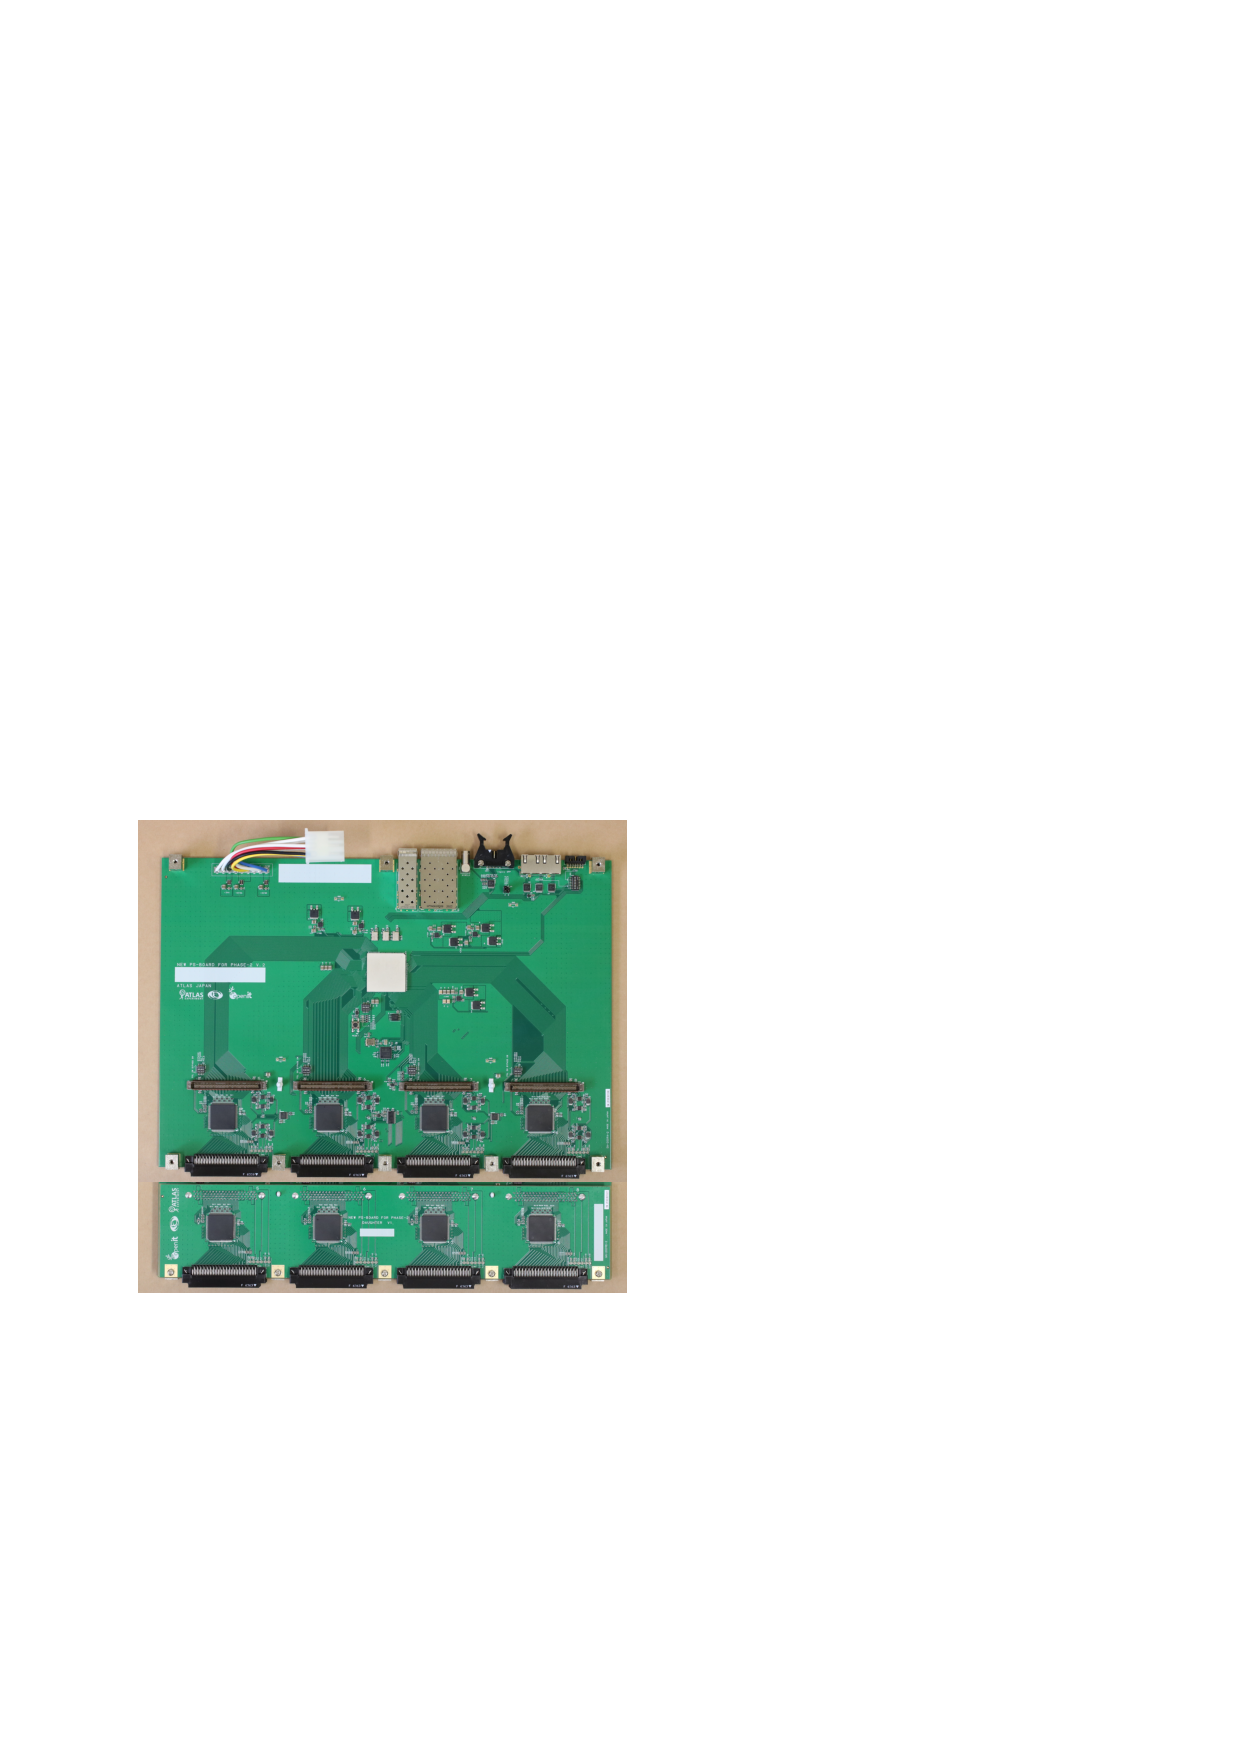
\includegraphics[height=8cm]{fig/Intro/TGC_PSB.pdf}
\subcaption{PS boardの写真}
\end{minipage}%
\begin{minipage}[b]{.5\linewidth}
\centering
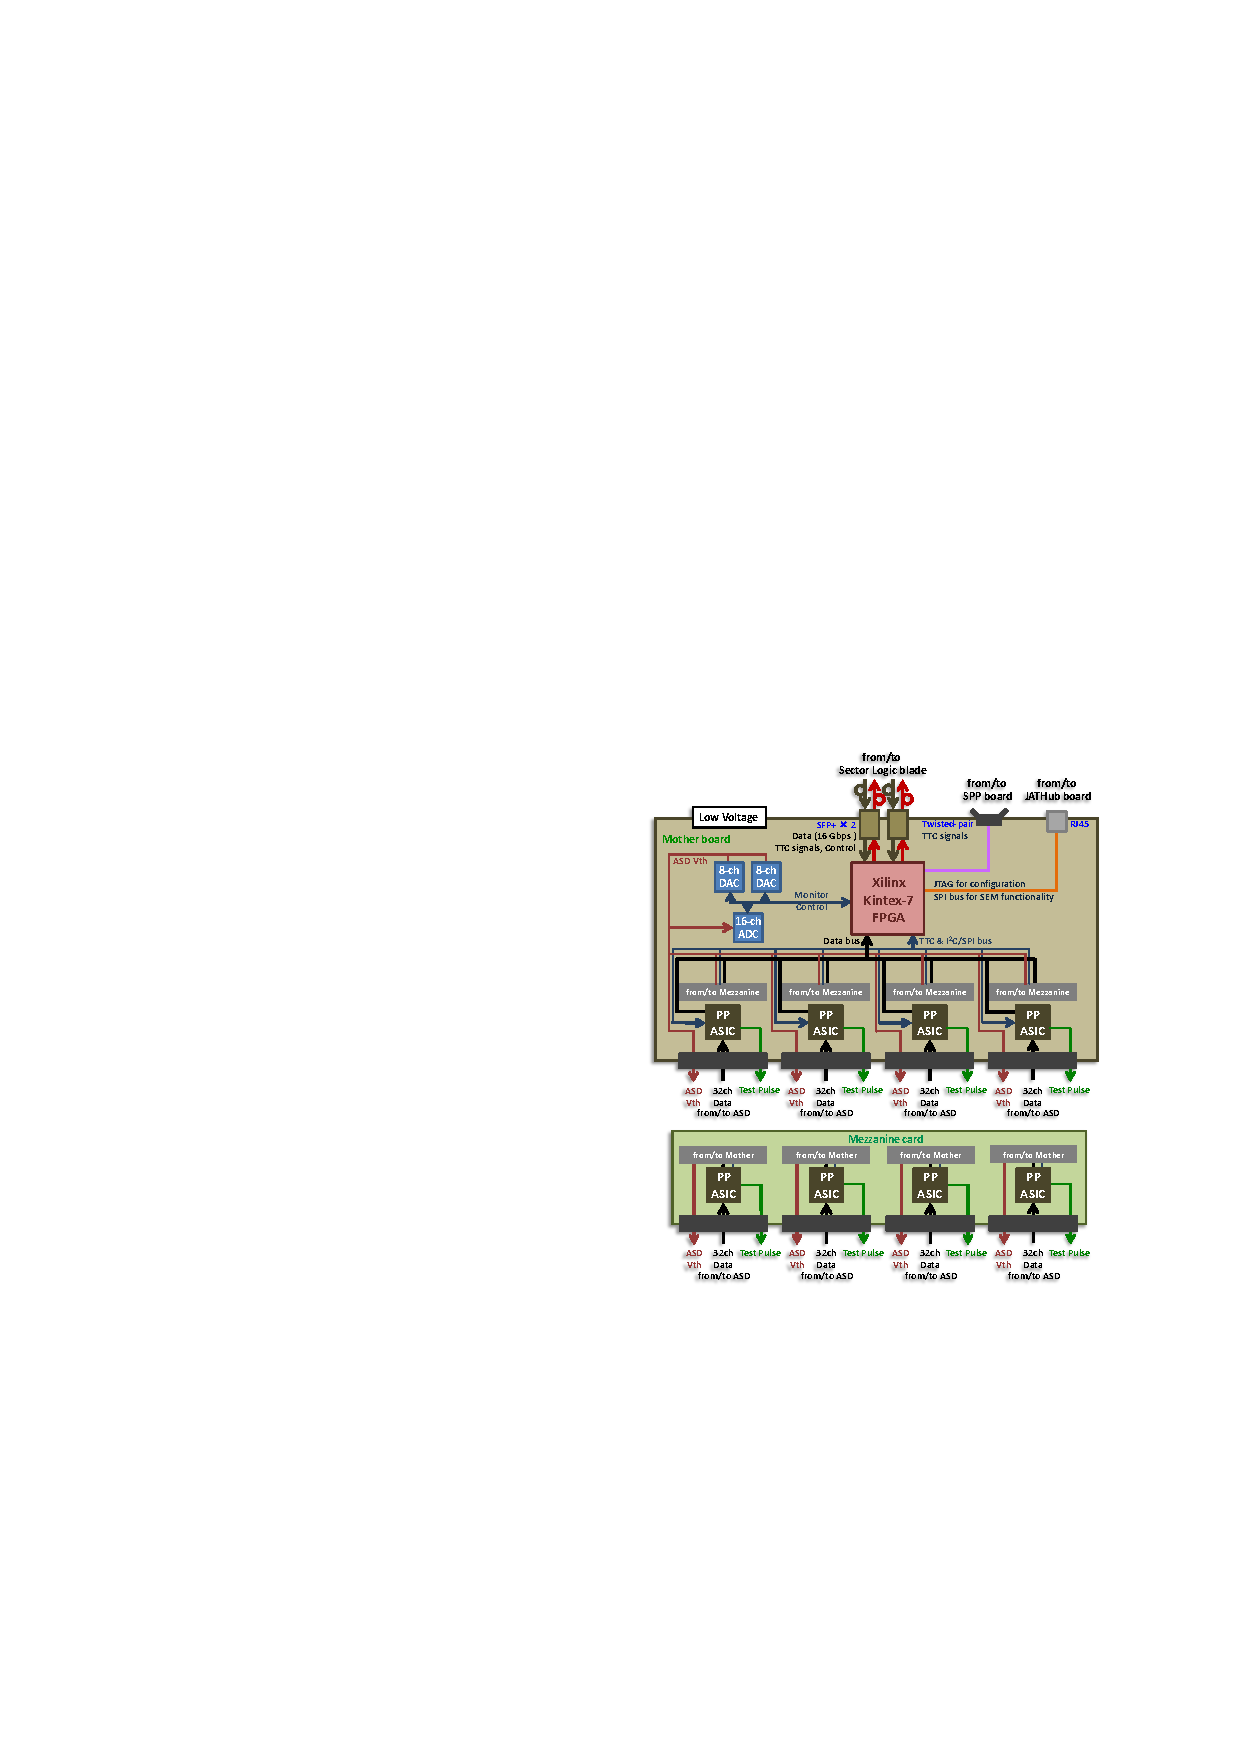
\includegraphics[height=8cm]{fig/Intro/TGC_PSBblock.pdf}
\subcaption{PS boardのブロック図}
\end{minipage}%
\caption[PS boardの概要]{PS boardの概要}
\label{TGC_PSB}
\end{figure}

\subsubsection*{Patch-Panel ASIC(PP ASIC)}
図\ref{}にPP ASICのブロック図を示す。PP ASICは主に可変遅延回路と陽子バンチ識別回路で構成される。

\begin{figure} 
\centering
\includegraphics[width=16cm]{fig/Intro/TGC_PPASIC.pdf}
\caption[PP ASIC回路のブロック図]{PP ASIC回路のブロック図\cite{PPASIC}}
\label{TGC_PPASIC}
\end{figure}

PP ASICが受け取るLVDS信号の入力時間は、チャンネルごとに最大26 ns程度のばらつきが存在する。これは、チャンネルごとにミューオンの衝突点から検出器までの飛行時間(Time-of-Flight)やASDからPP ASICまでのLVDSケーブルの長さが異なるからである。また、TGCの同一のチャンネルであってもイベント毎に信号到着時間が20 ~ 30 nsバラつく。(\ref{}参照)これはミューオンの入射位置によって、チェンバー内で電荷が検出される位置からASDまでの距離や、電荷のドリフト時間が変わるからである。

このばらつきを揃えるために、各ASDごとに固有の遅延をかけるのが可変遅延回路である。可変遅延回路は1ns以下の刻み幅で、最大45 nsの遅延をかけることができる。PP ASICに到着するのが一番遅いASDからの信号の立ち上がりに、他のASDからの信号の立ち上がりを揃えるように遅延パラメーターを設定する。この遅延パラメーターはPS boardのFGPAから設定することができる。

可変遅延回路でタイミングが揃えられた信号は、次に陽子バンチ識別回路に入る。陽子バンチ識別回路は、PP ASICに入射するデジタル信号の立ち上がりを検出し、その信号がどの陽子バンチ衝突に由来するのか識別する。陽子バンチ回路の概念図を図\ref{TGC_BCID}に示す。上述したように同じチャンネル内でもヒット信号の到着時間はイベント毎に20 ~ 30 ns程度の幅を持ち、この時間幅のうちに来るヒット信号には同じBCIDを付与する必要がある。そのため、同じBCIDを付与する時間幅(有効ゲート幅)をASDごとに設定できるようになっており、信号到着時間幅が25 nsを超える場合に対応するため、有効ゲート幅は25 nsを超えて設定できるようになっている。この場合、図\ref{TGC_BCID}のピンク色で囲まれた領域が示すように、2つの有効ゲートが重なる時間が存在するが、このタイミングに入射した信号に対しては2バンチ分の信号を出力する。有効ゲート幅もPS boardのFPGAから設定することができる。

\begin{figure} 
\centering
\includegraphics[width=16cm]{fig/Intro/TGC_BCID.pdf}
\caption[陽子バンチ識別回路のタイミングチャート]{陽子バンチ識別回路のタイミングチャート\cite{mt_takemoto}}
\label{TGC_BCID}
\end{figure}

\subsubsection*{PS board FPGA}
PS board FPGAはSLへヒットデータを転送することに加え、PS board上の各素子の制御及びLHCバンチ交差クロックの再構成を担う。

8つのPP ASICでLHC バンチ交差クロックと同期された256チャンネルのヒット信号はPS board上のFPGAでまとめられ、光ファイバーを経由してSLに転送される。

PS boardからSLに送られるデータフォーマットを図\ref{TGC_PSBuplink}に示す。256チャンネルのヒットデータに加え、64 bitのヘッダーが付与され合計320bitのデータが25 nsおきに送信される。320 bit のデータは2本の光ファイバーに分けられ、32bitごとにワードという塊を形成して送られる。ここでワード0ではヘッダーが、ワード1 ~ 4にヒットデータが詰められる。データ転送には高速シリアル通信に対応したGTXトランシーバーを用いる。ここでは8b10bコーディングを用いてFPGA内のパラレルデータからシリアルデータに変換するため、1本の光リンクのラインレートは$160 bit \times 10/8 \times 40 \mathrm{\,MHz} = 8Gbps$となる。

\begin{figure} 
\centering
\includegraphics[width=16cm]{fig/Intro/TGC_PSBuplink.pdf}
\caption[PS boardからSLへ送るデータフォーマット]{PS boardからSLへ送るデータフォーマット\cite{mt_aoki}}
\label{TGC_PSBuplink}
\end{figure}

また、PS board FGPAはSLからコントロール用の信号を1本の光ファイバー経由で受け取る。SLからPS boardに送られるデータフォーマットを図\ref{TGC_PSBdownlink}に示す。SLはワード2,3で定義されたAddress、Data、Command、データを利用しPS board FGPA内のレジスタを操作する。またPS board FPGAとQSPIフラッシュメモリーはSPIバスで繋がれており、SLからFPGAを経由してSPIバスをビットバンギングすることでQSPIフラッシュメモリーにデータを書き込むことができる。このパスを利用して、PPASICの遅延パラメーターや有効ゲート幅、ASDに供給する閾値電圧など、各PS board毎に異なるパラメーターがQSPIフラッシュメモリーに書き込まれる。

\begin{figure} 
\centering
\includegraphics[width=16cm]{fig/Intro/TGC_PSBdownlink.pdf}
\caption[SLからPS boardへ送るコントロールデータのフォーマット]{SLからPS boardへ送るコントロールデータのフォーマット\cite{mt_aoki}}
\label{TGC_PSBdownlink}
\end{figure}

TTC信号もこのコントロール線に乗せられてPS boardに分配される。PS boardのGTXトランシーバーはワード0で定義されたComma ワードを利用して、シリアルデータからLHCバンチ交差クロックを再構成する。PS boardで再構成されたLHCバンチ交差クロックは適切な遅延をかけられてから、ジッタークリーナーを通りFPGAやGTXトランシーバー、PPASICに分配される。

    \subsection*{JTAG AssisTance Hub(JATHub)}
JATHubはデータパスとは独立した、PS board制御用回路である。JATHubはPS board FPGAを常時モニターしており、PS board FPGAに修復不可能なSingle Event Upset(SEU)が生じた場合に、再コンフィギュレーション用の信号を送る。またPS board QSPIフラッシュメモリへのファームウェアの書き込み、LHCバンチ交差クロックの位相測定を行う。

概要を図\ref{TGC_JATHub}に示す。JATHubはプロセッサーとFPGAを組み合わせたXilinx社製のZynq SoCをメインドライバーとして搭載する。Zynqはプロセッサー部分であるProcessing System (PS)と、FPGA部分であるProgrammable Logic(PL、FPGA部分)で構成される。PS 部分にはLinuxを起動し、PS、PL間通信を利用してFPGAを操作することができる。

\begin{figure} 
\centering
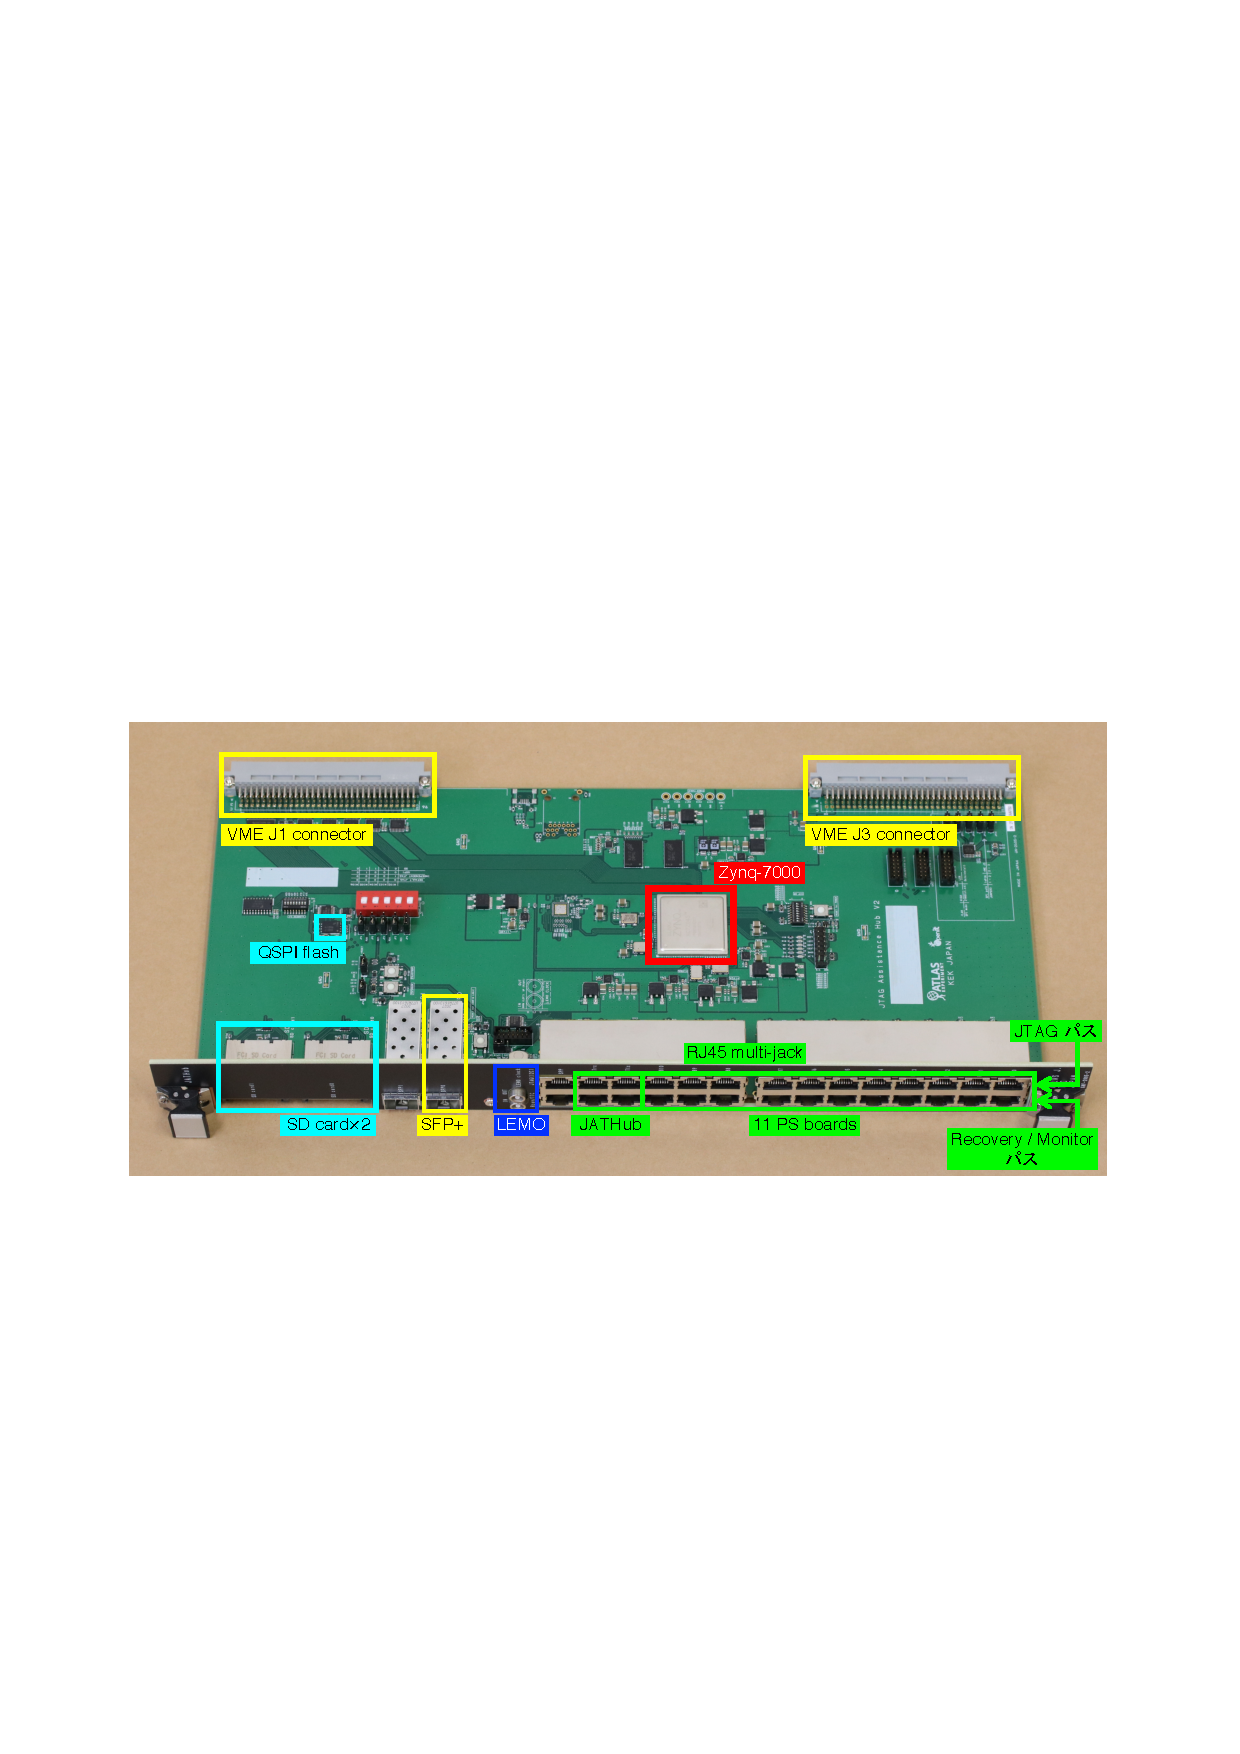
\includegraphics[width=16cm]{fig/Intro/TGC_JATHub.pdf}
\caption[JATHubの概要]{JATHubの概要}
\label{TGC_JATHub}
\end{figure}

インターフェイスとして、PS boardと接続するためのRJ45コネクター、ATLAS回路室とイーサーネット通信を行うためのSFP+モジュールを搭載している。JATHub 1枚で最大11枚のPS boardと接続され、それぞれ2本のCat-6ケーブルで接続される。

1本のCat-6ケーブルはJTAGパスと呼ばれ、PS board QSPIフラッシュメモリーにファームウェアを書き込むのに使われる。もう一本はRecovery/Monitorパスと呼ばれ、PS boardの再コンフィギュレーションやPS board上のバンチ交差クロックをJATHubに送るために利用される。

    \subsection*{Sector Logic(SL)}
PS board FPGAでまとめられた256チャンネル分のヒットデータはSLに入る。SLはVirtex UltraScale+ FPGAという大規模FPGAとZynq UltraScale+ MPSoCという2つの集積回路を搭載している。UltraScale+FPGAはSL FPGAと呼ばれ、PS boardから受信したヒットデータを用いてトリガー演算を行う。SL FPGAはCTPからL0Aが発行されるまでのデータのバッファーおよび後段への読み出しも担当する。Zynq UltraScale+ MPSoCはVirtexUltraScale+ FPGAやPS boardのコントロールマスターとして機能する。

SLの第一試作機の写真を図\ref{TGC_SL}に示す。

\begin{figure} 
\centering
\includegraphics[width=16cm]{fig/Intro/TGC_SL.jpg}
\caption[SL第一試作機の写真]{SL第一試作機の写真}
\label{TGC_SL}
\end{figure}

SLはAdvanced Telecommunications Computing Architecture(ATCA)規格のボードである。ユーザーはATCAクレートのShelf managerからCERNで開発されたIntelligent Platform Management Controller(IPMC)を介して、SLの電源や電圧のモニター、遠隔での電源操作を行うことができる。また外部とのインターフェイスとして電気信号を光信号に変換するためのFireFlyを送信用に10個、受信用に10個搭載している。それぞれが12リンクを束ねているため、送受信120リンクの光通信が可能である。LANケーブルのインターフェイスであるRJ45コネクターも搭載しており、ethernetを経由したネットワーク通信を行うことができる。

1枚のSLはTGCの1/24セクターからの信号処理を担当し、合計31台のPS boardと接続する(BW用に29 枚、EI用に2 枚)。A side、Cside合わせて合計で48枚のSLが設置される。以下にそれぞれのモジュールの機能の詳細を述べる。

    \subsubsection{SL FPGA}
SL FPGAに実装するファームウェアの概要を図\ref{}に示す。ファームウェアは大別してトリガー回路、読み出し回路、コントロールパスに分けられる。PS boardから光リンクを経由して送られるヒット情報は、トリガー回路および読み出し回路に入れられる。

\begin{figure} 
\centering
\includegraphics[width=16cm]{fig/Intro/SL_FW_overview.pdf}
\caption[SL FPGAに実装されるファームウェアの概要]{SL FPGAに実装されるファームウェアの概要\cite{}}
\label{fig_CTA}
\end{figure}

トリガー回路はPS boardから送られるBW 7層分のヒットデータを用いてpt判定を行なった後、エンドキャップトロイド磁石より内側のNSW、RPC BIS78、TIleカロリメーターから受信した情報も用いてより精度の高いpt概算を行う。実装されたトリガーロジックの詳細は次節で述べる。トリガー回路の出力情報はMUCTPIへ転送するとともに、モニターのためトリガー読み出し回路に入れられる。

読み出し回路はPS board から送られてきたヒットデータと、そのイベントに対するトリガーデータをバッファーしておき、L0A が発行されたイベントのデータを選択的に後段へ転送する役割を担う。読み出されるデータにはZerosuppressという圧縮処理が行われ、全PS board分のデータをイベントごとにパッキング(Event Building)した後FELIXへ送られる。

コントロールパスはSL FPGA内のコンフィギュレーションやパラメーター制御、などLHC バンチ交差クロックと同期する必要のないスローな制御を担当する。コントロールマスターのMPSoCからSL FPGA内のレジスタを操作することで、SLのトリガー・読み出しに関連するパラメーターの設定や、PS boardの制御を行う。

    \subsubsection*{Zynq MPSoC}
Zynq MPSoCは図\ref{}に示すようにProcessing System (PS)とProgrammable Logic(PL)から構成される。PSにはプロセッサやメモリが搭載されていて、標準的なOSであるcentos 7を起動する。ユーザーはネットワークを経由してSLにアクセスし、PSとPL間の通信を介してPLを操作することができる。また、Zynq MPSoCのPLとSL FPGAはGTHトランシーバーを介したチップ間通信が可能となっており、PSからSL FPGAを操作することができる。また、Zynq MPSOはTDAQシステムやDetector Control System(DCS)とのインターフェイスとなる。
